\documentclass[letterpaper, 11pt, oneside]{book}

\usepackage{style}  % If you feel like procrastinating, mess with this file
\usepackage{algo}   % Thank you Jeff, very cool!

\addbibresource{refs.bib}

% Required reading
% https://jmlr.csail.mit.edu/reviewing-papers/knuth_mathematical_writing.pdf
%   Along with required viewing:
%   https://www.youtube.com/watch?v=N6QEgbPWUrg&list=PLOdeqCXq1tXihn5KmyB2YTOqgxaUkcNYG
% https://faculty.math.illinois.edu/~west/grammar.html

% % % % % % % % % %
%     Cursor      %
%     Parking     %
%     Lot         %
% % % % % % % % % %

% Disable check for mismatched parens/brackets/braces
%   chktex-file 9
% Disable check for different counts of parents/brackets/braces
%   chktex-file 17
% Exclude these environments from syntax checking
%   VerbEnvir { tikzcd }

\regtotcounter{figure}

\title{\vspace{-100pt} 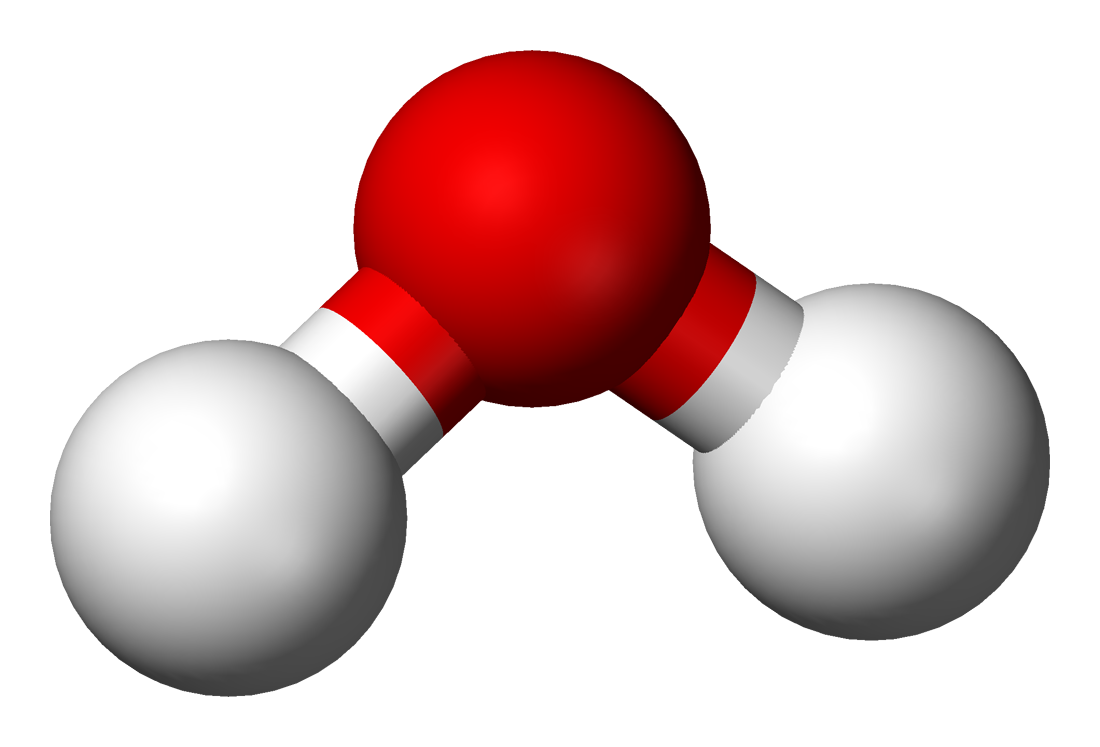
\includegraphics[width=0.75\textwidth]{figs/water.png} \\ {\Huge Representation Theory Notes and Exercises} \\ {\small With $\total{figure}$ Figures}}
\author{\Large Anakin Dey}
\DTMsavenow{now}
\date{\small Last Edited on \today\ at \DTMfetchhour{now}:\DTMfetchminute{now}}

% Cover page number chicanery
\newcommand{\CoverName}{Cover}

\begin{document}
\frontmatter
\renewcommand{\thepage}{\CoverName}
\maketitle

\pagenumbering{roman}

\section*{TODOs}

\quest{Change the style of enumerates from ``1.'' to ``(1)''}

\quest{Proper Exercise Header}

\quest{Proper Chapter Header}

\quest{Remove indent at end of thmtool environments}

\tableofcontents
\clearpage


\listoftheorems[ignoreall, show={defn}, title={List of Definitions}]

\listoftheorems[ignoreall, show={ex}, title={List of Examples and Counterexamples}]

\chapter*{Preface}

This is a set of notes on group representation theory mainly based on J.P. Serre's text \emph{Linear Representations of Finite Groups}~\cite{book:SerreLinReps}.
Occasionally, other sources may be used, such as the set of notes by Charles Rezk created for Math 427~\cite{note:rezk_reps}.
The goal of these notes is to eventually work towards algebraic combinatorics such as Fulton's text \emph{Young Tableaux}~\cite{book:FultonTableaux}, as much of algebraic combinatorics is motivated by questions stemming from representation theory.
At the time of writing this, another goal is the applications of representation theory to computational complexity: see~\cite{misc:PanovaComputational} for a recent survey on this connection.

\mainmatter

\chapter{Generalities on Linear Representations}

Unless otherwise specified, $V$ will denote a vector space, usually over the field $\C$.
We will restrict ourselves to finite dimensional vector spaces.
Similarly, we will restrict ourselves to finite groups.

\begin{defn}[Linear Representation, Representation Space]
  Let $G$ be a group with identity $e$.
  A \emph{linear representation} of $G$ in $V$ is a homomorphism $\rho\colon G \to \GL(V)$.
  We will frequently, and often interchangeably, write $\rho_{s} \defeq \rho(s)$.
  Given $\rho$, we will say that $V$ is a \emph{representation space} or \emph{representation} of $G$.
\end{defn}

\begin{defn}[Degree]
  Let $\rho\colon G \to V$ be a representation of $G$ in a vector space $V$.
  Then the \emph{degree} of $\rho$ is $\dim(V)$.
\end{defn}

Let $\rho\colon G \to V$ be a representation of $G$ in a vector space $V$ with $n \defeq \dim(V)$.
Fix a basis $(e_{j})$ of $V$.
Then since each $\rho_{s}$ is an invertible linear transformation of $V$, we may define an $n \times n$ matrix $R_{s} \equiv (r_{ij}(s))$ where each $r_{ij}(s)$ is defined by the identity
\[
  \rho_{s}(e_{j}) = \sum_{i = 1}^{n} r_{ij}(s) e_{i}.
\]

\begin{defn}[Matrix of a Representation]
  We call $R_{s} = (r_{ij}(s))$ above the \emph{matrix of $\rho_{s}$} with respect to the basis $(e_{j})$.
\end{defn}
Note that $R_{s}$ satisfies the following:
\begin{align*}
  \det(R_{s}) \neq 0, && R_{st} = R_{s} \cdot R_{t} \equiv r_{ij}(st) = \sum_{k = 1}^{n} r_{ik}(s) \cdot r_{kj}(s) \quad \forall s, t \in G.
\end{align*}

\clearpage

Recall that two $n \times n$ matrices $A, A'$ are \emph{similar} if there exists an invertible matrix $T$ such that $T A = A' T$.
We may extend this notion to representations.
\begin{defn}[Similar/Isomorphic Representations]
  Let $\rho$ and $\rho'$ be two representations of the same group $G$ in vector spaces $V$ and $V'$ respectively.
  We say $\rho$ and $\rho'$ are \emph{similar} or \emph{isomorphic} if there exists an isomorphism $\tau \colon V \to V'$ such that for all $s \in G$, $\tau$ satisfies $\tau \circ \rho(s) = \rho'(s) \circ \tau$.
  If $R_{s}, R'_{s}$ are the corresponding matrices then this is equivalent to saying there exists an invertible matrix $T$ such that $T R_{s} = R'_{s} T$ for all $s \in G$.
\end{defn}
Note that if $\rho$ and $\rho'$ are isomorphic, then they must have the same degree.

We now give some examples of these things.
\begin{ex}[Unit/Trivial Representation]\label{ex:unit_trivial_representation}
  Let $G$ be a finite group.
  Representations of degree $1$ must be of the form $\rho\colon G \to \C^{\times}$.
  Since elements $s$ of $G$ are of finite order, $\rho(s)$ must also be of finite order.
  Thus, for all $s \in G$, $\rho(s)$ is a root of unity.
  If we take $\rho(s) = 1$ for all $s \in G$, we obtain the \emph{unit} or \emph{trivial} representation of $G$.
  This also means that $R_{s} = 1$ for all $s$.
\end{ex}

\begin{ex}[Regular Representation]\label{ex:regular_representation_Z3}
  Let $g$ be the order of $G$, and let $V$ be a vector space of dimension $g$ with a basis $(e_{t})_{t \in G}$.
  For each $s \in G$, define $\rho_{s}$ as the linear map $\rho_{s}\colon V \to V$ such that $\rho_{s}(e_{t}) = e_{st}$.
  This is a linear representation of $G$ called the \emph{regular} representation of $G$.
  Since for each $s \in G$, $e_{s} = \rho_{s}(e_{1})$ and thus the images of $e_{1}$ form a basis of $V$.
  Conversely, let $W$ be a representation of $G$ with a vector $w$ satisfying the collection of all $\rho_{s}(w)$, $s \in G$, forms a basis of $W$.
  Then $W$ is isomorphic to the regular representation of $G$ by the isomorphism $\tau(e_{s}) = \rho_{s}(w)$.

  For example, let $G = \Z_{3}$ and $V = \C^{3}$ with $e_{0} = (1, 0, 0)$, $e_{1} = (0, 1, 0)$, and $e_{2} = (0, 0, 1)$.
  Then for example, $\rho_{0}, \rho_{1}, \rho_{2}\colon \C^{3} \to \C^{3}$ are the linear maps such that
  \begin{align*}
    \rho_{0}(e_{0}) = e_{0 + 0} = e_{0} && \rho_{0}(e_{1}) = e_{0 + 1} = e_{1} && \rho_{0}(e_{2}) = e_{0 + 2} = e_{2} \\
    \rho_{1}(e_{0}) = e_{1 + 0} = e_{1} && \rho_{1}(e_{1}) = e_{1 + 1} = e_{2} && \rho_{1}(e_{2}) = e_{1 + 2} = e_{0} \\
    \rho_{2}(e_{0}) = e_{2 + 0} = e_{2} && \rho_{2}(e_{1}) = e_{2 + 1} = e_{0} && \rho_{2}(e_{2}) = e_{2 + 2} = e_{1}
  \end{align*}
  With this, the matrix representations of $\rho_{0}, \rho_{1}$ and $\rho_{2}$ is similarly straightforward:
  \begin{align*}
    R_{0} = \begin{pmatrix} 1 & 0 & 0 \\ 0 & 1 & 0 \\ 0 & 0 & 1 \end{pmatrix} && R_{1} = \begin{pmatrix} 0 & 0 & 1 \\ 1 & 0 & 0 \\ 0 & 1 & 0 \end{pmatrix} && R_{2} = \begin{pmatrix} 0 & 1 & 0 \\ 0 & 0 & 1 \\ 1 & 0 & 0 \end{pmatrix}
  \end{align*}
\end{ex}

\clearpage

\begin{ex}[Permutation Representation]
  We may generalize the regular representation to any group action $G \acts X$, $X$ a finite set.
  Recall that for such an action, the map $x \mapsto sx$ for each $s \in G$ is a permutation $X \tofrom X$.
  Let $V$ be a vector space with dimension the size of $X$, and so a basis $(e_{x})_{x \in X}$.
  Define a representation $\rho$ of $G$ by defining $\rho_{s}$ as the linear map sending $e_{x} \mapsto e_{sx}$.
  This representation is known as the \emph{Permutation} representation of $G$ associated with $X$.
  If we consider $X = [n]$ and $G = S_{n}$, then take $V = \C^{n}$ as our vector space and $e_{i}$ as the standard basis vector.
  Then $\rho_{\sigma}(e_{j}) = e_{\sigma_{j}}$.
  Thus for each $\sigma \in S_{n}$, we have that $R_{\sigma} = (r_{ij}(\sigma))$ where entry $r_{ij}(\sigma) = 1$ if $i = \sigma_{j}$ and $0$ otherwise.
\end{ex}

\begin{defn}[Stable/Invariant Subspaces, Subrepresentation]
  Let $\rho\colon G \to \GL(V)$ be a linear representation and $W \subseteq V$ a subspace of $V$.
  We say that $W$ is \emph{stable} under the action of $G$ if $x \in W$ implies that $\rho_{s}(x) \in W$ for all $s \in G$.,
  Thus, the restriction $\rho_{s}^{W} \defeq \rho_{s}\mid_{W}$ is an isomorphism of $W$ onto itself.
  Restrictions satisfy the property that $\rho_{s}^{W} \circ \rho_{t}^{W} = \rho_{st}^{W}$.
  Thus, $\rho^{W}\colon G \to \GL(W)$ is a linear representation of $G$ in $W$ and we say that $W$ is a \emph{subrepresentation} of $V$.
\end{defn}

\begin{ex}[Subrepresentations of the Regular Representation]\label{ex:subrep_reg_rep}
  Let $G$ be a group.
  Recall the regular representation $V$ given in \Cref{ex:regular_representation_Z3}.
  Let $W$ be the 1 dimensional subspace of $V$ generated by the element $x = \sum_{s \in G} e_{s}$.
  Then note that $\rho_{s}(x) = x$ for all $s \in G$ and thus $W$ is a subrepresentation of $V$.
  Furthermore, this is isomorphic to the unit representation \Cref{ex:unit_trivial_representation} with $\tau\colon C^{\times} \to W$ such that $\tau(1) = x$.
  For example, let $G = \Z_{3}$ and $\rho\colon \Z_{3} \to \GL(\C^{3})$ the representation given in \Cref{ex:regular_representation_Z3}.
  Then $x = (1, 1, 1)$ and for example we have that
  \[
    \rho_{1}(x) = \rho_{1}(e_{0}) + \rho_{1}(e_{1}) + \rho_{1}(e_{2}) = e_{1} + e_{2} + e_{0} = x.
  \]
\end{ex}

\begin{thrm}\label{thrm:stable_complements_of_subspace}
  Let $\rho\colon G \to \GL(V)$ be a linear representation of $G$ in $V$ and let $W$ be a subspace of $V$ stable under $G$.
  Then there exists a complement $W^{0}$ of $W$ in $V$ which is stable under $G$.
\end{thrm}
\begin{pf}
  Let $W'$ be an arbitrary complement of $W$ in $V$, and let $p\colon V \to W$ be the projection.
  Then we form the average $p^{0}$ of conjugates of $p$ by elements in $G$:
  \[
    p^{0} \defeq \frac{1}{\abs{G}} \sum_{t \in G} \rho_{t} \circ p \circ \rho_{t}^{-1}.
  \]
  Since $p\colon V \to W$ and $\rho_{t}$ preserves $W$, we have that $p^{0}$ maps $V$ onto $W$.
  Furthermore, note that $\rho_{t}^{-1}$ also preserves $W$.
  \clearpage
  Thus we have that
  \begin{align*}
    (p \circ \rho_{t}^{-1})(x) = \rho_{t}^{-1}(x), && (\rho_{t} \circ p \circ \rho_{t}^{-1})(x) = x, && p^{0}(x) = x.
  \end{align*}
  Thus, $p^{0}$ is a projection of $V$ onto $W$, corresponding to some complement $W^{0}$ of $W$.
  Moreover, we have that $\rho_{s} \circ p^{0} = p^{0} \circ \rho_{s}$ for all $s \in G$ because
  \[
    \rho_{s} \circ p^{0} \circ \rho_{s}^{-1} = \frac{1}{\abs{G}} \sum_{t \in G} \rho_{s} \circ \rho_{t} \circ p \circ \rho_{t}^{-1} \circ \rho_{s}^{-1} = \frac{1}{\abs{G}} \sum_{t \in G} \rho_{st} \circ p \rho_{st}^{-1} = p^{0}.
  \]
  Now suppose that $x \in W^{0}$ and $s \in G$, we have that $p^{0}(x) = 0$ and hence $(p^{0} \circ \rho_{s})(x) = (\rho_{s} \circ p^{0})(x) = 0$, meaning that $\rho_{s}(x) \in W^{0}$.
  This, $W^{0}$ is stable under $G$.
\end{pf}

Suppose that $V$ had an innerproduct $\inner{x, y}$, and furthermore suppose this inner product was invariant under $G$ meaning that for all $s \in G$, $\inner{\rho_{s}(x), \rho_{s}(y)} = \inner{x, y}$.
We may also reduce to this case by replacing $\inner{x, y}$ with $\sum_{t \in G}\inner{\rho_{t}(x), \rho_{t}(y)}$.
With this, the orthogonal complement $W^{\bot}$ of $W$ in $V$ is a complement of $W$ stable under $G$.
Note that the invariance of $\inner{x, y}$ means that if $(e_{i})$ is an orthonormal basis of $V$, then $R_{s}$ is a unitary matrix.

Using the notation of \Cref{thrm:stable_complements_of_subspace}, let $x \in V$ and $w, w^{0}$ be the projections of $x$ on $W$ and $W^{0}$ respectively.
Thus for all $s \in G$, $\rho_{s}(x) = \rho_{s}(w) + \rho_{s}(w^{0})$.
Since $W$ and $W^{0}$ are stable under $G$, we have that $\rho_{s}(w) \in W$ and $\rho_{s}(w^{0}) \in W^{0}$.
This means that $\rho_{s}(w)$ and $\rho_{s}(w^{0})$ are the projections of $\rho_{s}(x)$ and in turn the representations of $W$ and $W^{0}$ determine the representations of $V$.
\begin{defn}[Direct Sum of Representations]
  Given the above, we write $V = W \oplus W^{0}$ as the \emph{direct sum} of $W$ and $W^{0}$.
  We identify elements $v \in V$ as pairs $(w, w^{0})$ given by their projections.
\end{defn}
If the representations $W$ and $W^{0}$ are given in matrices $R_{s}$ and $R_{s}^{0}$, then the matrix form of the representation $V$ is given by
\[
  \begin{pmatrix} R_{s} & 0 \\ 0 & R_{s}^{0} \end{pmatrix}.
\]
Similar results hold for arbitrarily many, but finite, direct sums of representations.

The above is a discussion on how to compose two or more representations into one larger representation.
The natural question is then about the opposite.
\begin{defn}[Irreducible/Simple Representations]
  Let $\rho\colon G \to \GL(V)$ be a linear representation of $G$.
  Then this representation is \emph{irreducible} or \emph{simple} if $V$ has no subspaces stable under $G$ besides $0$ and $V$ itself.
\end{defn}
By \Cref{thrm:stable_complements_of_subspace}, this is equivalent to saying that $V$ is not the direct sum of two representations besides $V = 0 \oplus V$.
A representation of degree $1$ is reducible.
We may use irreducible representations to construct other ones via the direct sum.

\begin{thrm}
  Every representation is a direct sum of irreducible representations.
\end{thrm}
\begin{pf}
  Let $V$ be a linear representation of $G$.
  We induct on $\dim(V)$.
  If $\dim(V) = 0$, then $V = 0$ which is the direct sum of an empty family of irreducible representations.
  So suppose that $\\dim(V) \geq 1$.
  If $V$ is irreducible, then we are done.
  Otherwise, there exists a subspace $W \subsetneq V$ stable under $G$ and by \Cref{thrm:stable_complements_of_subspace} a stable complement $W^{0}$ such that $V = W \oplus W^{0}$.
  By assumption, $W \neq 0 \neq W^{0}$ and so $\dim(W) < V$ and $\dim(W^{0}) < \dim(V)$.
  By induction, we have obtained a decomposition of $V$ into irreducibles.
\end{pf}

\begin{ex}[Decomposition of Representation of $\Z_3$ into Irreducibles]
  Recall from \Cref{ex:regular_representation_Z3} the regular representation $\rho\colon \Z_{3} \to \GL(\C^{3})$ with $e_{0} = (1, 0, 0)$, $e_{1} = (0, 1, 0)$, and $e_{2} = (0, 0, 1)$ and
  \begin{align*}
    \rho_{0}(e_{0}) = e_{0} && \rho_{0}(e_{1}) = e_{1} && \rho_{0}(e_{2}) = e_{2} \\
    \rho_{1}(e_{0}) = e_{1} && \rho_{1}(e_{1}) = e_{2} && \rho_{1}(e_{2}) = e_{0} \\
    \rho_{2}(e_{0}) = e_{2} && \rho_{2}(e_{1}) = e_{0} && \rho_{2}(e_{2}) = e_{1}
  \end{align*}
  Our goal will be to decompose $\rho$ into $\rho^{1} \oplus \rho^{2} \oplus \rho^{3}$.
  We aim to find the elements fixed by $\Z_{3}$.
  Note that if an element is fixed by $1$, the generator of $\Z_{3}$, then it is fixed by all of $\Z_{3}$.
  We want to find 1-dimensional $\Z_3$-invarient subspaces of $\C^{3}$.
  This is equivalent to finding the eigenvalues of the matrix
  \[
    R_{1} = \begin{pmatrix} 0 & 0 & 1 \\ 1 & 0 & 0 \\ 0 & 1 & 0 \end{pmatrix}.
  \]
  The eigenvalues their eigenvectors of $R_{1}$ are as follows, note the inclusion of the trivial subrepresentation from \Cref{ex:subrep_reg_rep}:
  \begin{align*}
    \lambda_{1} = 1, v_{1} = \begin{pmatrix} 1 \\ 1 \\ 1 \end{pmatrix} && \lambda_{2} = \frac{-1 -i \sqrt{3}}{2}, v_{2} = \begin{pmatrix} \frac{-1 + i \sqrt{3}}{2} \\ \frac{-1 -i \sqrt{3}}{2} \\ 1 \end{pmatrix} && \lambda_{3} = \frac{-1 + i \sqrt{3}}{2}, v_{3} = \begin{pmatrix} \frac{-1 - i \sqrt{3}}{2} \\ \frac{-1 + i \sqrt{3}}{2} \\ 1 \end{pmatrix}
  \end{align*}
  Thus $\C^{3} = V_{1} \oplus V_{2} \oplus V_{3}$ where $V_{i} \defeq \vspan(v_{i})$.
  Note that there are only 3 morphisms $\Z_{3} \to \C^{\times}$ mapping $1$ to $1$, $\omega$, or $\omega^{2}$ where $\omega$ is a cube root of unity.
  Thus $\rho^{1}, \rho^2$, and $\rho^{3}$ must correspond to these morphisms \quest{but which ones}.
\end{ex}

A natural question is if such a decomposition $V = W_{1} \oplus \cdots \oplus W_{k}$ is unique.
However, suppose that $\rho$ is the trivial representation (\Cref{ex:unit_trivial_representation}).
Then each component of the decomposition is a line and we can decompose a vector space into the direct sum of lines in a number of ways.
However, we will see that the number of $W_{i}$ that are isomorphic to a given irreducible representation does not depend on the choice of decomposition.

\begin{defn}[Tensor/Kronekcer Product of Representations]
  Let $\rho^{1}\colon G \to \GL(V_{1})$ and $\rho^{2}\colon G \to \GL(V_{2})$ be two representations of a group $G$.
  We construct a representation $\rho\colon G \to \GL(V_{1} \otimes V_{2})$ such that
  \[
    \rho_{s}(x_{1} \otimes x_{2}) = \rho_{s}^{1}(x_{1}) \circ \rho_{s}^{2}(x_{2}) \quad \text{for } x_{1} \in V_{1}, x_{2} \in V_{2}.
  \]
  The existence and uniqueness of $\rho$ follow immediately from the existence and uniqueness of the tensor product.
  We write $\rho_{s} \equiv \rho_{s}^{1} \otimes \rho_{s}^{2}$ as the \emph{tensor product} of the given representations.
\end{defn}

Recall that if $(e_{i_{1}})$ and $(e_{i_{2}})$ be bases of $V_{1}$ and $V_{2}$ respectively, then $(e_{i_{1}} \otimes e_{i_{2}})$ is a basis of $V_{1} \otimes V_{2}$.
If $(r_{i_{1}j_{1}}(s))$ and $(r_{i_{2}j_{2}}(s))$ are the matrices of $\rho_{s}^{1}$ and $\rho_{s}^{2}$ respectively satisfying
\begin{align*}
  \rho_{s}^{1}(e_{j_{1}}) = \sum_{i_{1}} r_{i_{1}j_{1}} e_{i_{1}} && \rho_{s}^{2}(e_{j_{2}}) = \sum_{i_{2}} r_{i_{2}j_{2}} e_{i_{2}}
\end{align*}
then the matrix of $\rho_{s}$ is $(r_{i_{1}j_{1}}(s) \cdot r_{i_{2}j_{2}}(s))$ satisfying
\[
  \rho_{s}(e_{j_{1}} \otimes e_{j_{2}}) = \sum_{i_{1}, i_{2}} r_{i_{1}j_{1}}(s) \cdot r_{i_{2}j_{2}}(s) \cdot e_{i_{1}} \otimes e_{i_{2}}.
\]
\quest{TODO: example of tensor product}
Note that the tensor product of two irreducible representations is not in general irreducible \quest{TODO: example?}.
% https://math.stackexchange.com/questions/3191043/example-of-tensor-product-of-two-representations

We now consider the special case of $V \otimes V$.
Let $(e_{i})$ be a basis of $V$ and define an automorphism $\theta$ of $V \otimes V$ such that $\theta(e_{i} \otimes e_{j}) = e_{j} \otimes e_{i}$.
Then note that $\theta^{2} \equiv \id_{V \otimes V}$.
We may decompose $V \otimes V$ into the direct sum
\[
  V \otimes V = \Sym^{2}(V) \oplus \Alt^{2}(V).
\]
Here, $\Sym^{2}(V)$ is the set of $z \in V \otimes V$ such that $\theta(z) = z$ and $\Alt^{2}(V)$ is the set of $z \in V \otimes V$ where $\theta(z) = -z$.
These have bases $(e_{i} \otimes e_{j} + e_{j} \otimes e_{i})_{i \leq j}$ and $(e_{i} \otimes e_{j} - e_{j} \otimes e_{i})_{i < j}$ respectively.
As such, $\dim(\Sym^{2}(V)) = \frac{n(n + 1)}{2}$ and $\dim(\Alt^{2}(V)) = \frac{n(n - 1)}{2}$ where $n \defeq \dim(V)$.

\begin{defn}[Symmetric Square, Alternating Square]\label{defn:sym_alt_square}
  These subspaces $\Sym^{2}(V)$ and $\Alt^{2}(V)$ of $V \otimes V$ are respectively called the \emph{symmetric square} and \emph{alternative square} of the given representation.
\end{defn}

\chapter{Character Theory}

\begin{defn}[Character]
  Let $\rho\colon G \to \GL(V)$ be a linear representation of a finite group $G$ in $V$.
  Then the \emph{character} $\chi_{\rho}$ of $\rho$ is the function
  \[
    \chi_{\rho}(s) \defeq \Tr(R_{s}) \equiv \Tr(\rho_{s}).
  \]
  for each $s \in G$.
\end{defn}

\begin{prop}
  If $\chi$ is the character of a representation $\rho$ of degree $n$ then
  \begin{enumerate}
  \item $\chi(e) = 1$;
  \item $\chi(s^{-1}) = \chi(s)^{*}$, the complex conjugate of $\chi(s)$,
  \item $\chi(tst^{-1}) = \chi(s)$.
  \end{enumerate}
\end{prop}
\begin{pf}
  The first is immediate since $\rho_{1}$ is the identity matrix $I$ and $\Tr(I) = n$.
  Then recall that we may choose our basis to be orthonormal, and as such $\rho_{s}$ is a unitary matrix.
  Thus, each eigenvalue $\lambda_{1}, \ldots, \lambda_{n}$ has an absolute value equal to $1$.
  Thus
  \[
    \chi(s)^{*} = \Tr(\rho_{s})^{*} = \sum \lambda_{i}^{*} = \sum \lambda_{i}^{-1} = \Tr(\rho_{s})^{-1} = \Tr(\rho_{s^{-1}}) = \chi(s^{-1}).
  \]
  This uses the fact that the conjugate of the sum is the sum of the conjugates as well as the fact that the eigenvalues of $R_{s}^{-1}$ are the inverses of the eigenvalues of $R_{s}$.
  Finally, letting $u = ts$ and $v = t^{-1}$ allows us to write $\chi(tst^{-1}) = \chi(s)$ as $\chi(uv) = \chi(vu)$ which is immediate since for any complex matrices $A, B$ we have that $\Tr(AB) = \Tr(BA)$.
\end{pf}

\clearpage

\begin{prop}
  Let $\rho^{1}\colon G \to \GL(V_{1})$ and $\rho^{2}\colon G \to \GL(V_{2})$ be two linear representations with characters $\chi_{1}$ and $\chi_{2}$ respectively.
  Then
  \begin{enumerate}
  \item The character $\chi$ of the direct sum representation $V_{1} \oplus V_{2}$ is $\chi_{1} + \chi_{2}$.
  \item The character $\psi$ of the tensor product representation $V_{1} \otimes V_{2}$ is $\chi_{1} \cdot \chi_{2}$.
  \end{enumerate}
\end{prop}
\begin{pf}
  Let $R_{s}^{1}, R_{s}^{2}$ be the matrix forms of $\rho^{1}_{s}$ and $\rho_{s}^{2}$ respectively.
  Then the matrix form $R_{s}$ of the representation of $V_{1} \oplus V_{2}$ is given by
  \[
    R_{s} = \begin{pmatrix} R_{s}^{1} & 0 \\  0& R_{s}^{2} \end{pmatrix}
  \]
  and thus $\Tr(R_{s}) = \Tr(R_{s}^{1}) + \Tr(R_{s}^{2})$.
  Let $(e_{i_{1}})$ and $(e_{i_{2}})$ be bases for $V_{1}$ and $V_{2}$.
  Then we have that
  \[
    \psi(s) = \sum_{i_{1} i_{2}} r_{i_{1}i_{1}}(s) \cdot r_{i_{2}i_{2}}(s) = \pqty{\sum_{i_{1}} r_{i_{1}i_{1}}(s)} \cdot \pqty{\sum_{i_{2}} r_{i_{2}i_{2}}(s)} = \chi_{1}(s) \cdot \chi_{2}(s).
  \]
\end{pf}

\begin{prop}
  Let $\rho\colon G \to \GL(V)$ be a linear representation of $G$ with character $\chi$.
  Let $\chi_{\sigma}^{2}$ be the character of $\Sym^{2}(V)$ and $\chi_{\alpha}^{2}$ be the character of $\Alt^{2}(V)$ from \Cref{defn:sym_alt_square}.
  Then
  \begin{align*}
    \chi_{\sigma}^{2}(s) &= \frac{1}{2}\pqty{\chi(s)^{2} + \chi(s^{2})} \\
    \chi_{\alpha}^{2}(s) &= \frac{1}{2}\pqty{\chi(s)^{2} - \chi(s^{2})}
  \end{align*}
  which directly implies that $\chi_{\sigma}^{2} + \chi_{\alpha}^{2} = \chi$.
\end{prop}

\clearpage

\begin{pf}
  Let $s \in G$ and $(e_{i})$ a basis of $V$ consisting solely of eigenvectors for $\rho_{s}$.
  Then $\rho_{s}(e_{i}) = \lambda_{i}e_{i}$ for some $\lambda_{i} \in \C$.
  Thus
  \begin{align*}
    \chi(s) = \sum \lambda_{i} && \chi(s^{2}) = \sum \lambda_{i}^{2}.
  \end{align*}
  We also have that
  \begin{align*}
    (\rho_{s} \otimes \rho_{s})(e_{i} \otimes e_{j} + e_{j} \otimes e_{i}) &= \lambda_{i}\lambda_{j}(e_{i} \otimes e_{j} + e_{j} \otimes e_{i}) \\
    (\rho_{s} \otimes \rho_{s})(e_{i} \otimes e_{j} - e_{j} \otimes e_{i}) &= \lambda_{i}\lambda_{j}(e_{i} \otimes e_{j} - e_{j} \otimes e_{i})
  \end{align*}
  which yields that
  \begin{align*}
    \chi_{\sigma}^{2}(s) &= \sum_{i \leq j} \lambda_{i} \lambda_{j} = \sum \lambda_{i}^{2} + \sum_{i < j} \lambda_{i} \lambda_{j} = \frac{1}{2}\pqty{\sum \lambda_{i}}^{2} + \frac{1}{2} \sum \lambda_{i}^{2}
    \chi_{\alpha}^{2}(s) &= \sum_{i < j} \lambda_{i} \lambda_{j} = \frac{1}{2}\pqty{\sum \lambda_{i}}^{2} - \frac{1}{2} \sum \lambda_{i}^{2}.
  \end{align*}
  The proposition then directly follows.
  Note that the equality $\chi_{\sigma}^{2} + \chi_{\alpha}^{2} = \chi^{2}$ directly reflects the fact that $V \otimes V = \Sym^{2}(V) \oplus \Alt^{2}(V)$.
\end{pf}

\clearpage

\section*{Exercises}

\printbibliography
\end{document}
